\section{Resultados}

    \par En todos los casos, se realizaron 10000 simulaciones para calcular la media
    y la desviación estándar. Con los resultados de estas simulaciones se
    contruyeron los distintos histogramas que se presentan a continuación.

    \par Dado el contexto del problema, resulta de gran interés saber cómo maximizar el
    tiempo que tarda el sistema en fallar. Para ésto, los parámetros más
    significativos son $S$ y $O$ ya que éstos son los que el dueño del
    local modficaría para maximizar sus ganancias.
    Es por ésto que los parámetros que se pusieron en comparación son los
    anteriormente nombrados.

    \par Los tres experimentos realizados utilizaron los siguientes parámetros:
        \begin{itemize}
            \item{2 máquinas de repuesto y 1 operario.}
            \item{2 máquinas de repuesto y 2 operarios.}
            \item{3 máquinas de repuesto y 1 operario.}
        \end{itemize}

    \par En los histogramas, el eje X representa el tiempo, en meses, en el que falla el
    sistema y el eje Y representa la frecuencia del tiempo que tarda el sistema en
    fallar.
    En la esquina superior derecha se puede observar la media y la desviación
    estándar resultante los experimentos.
    Adicionalmente, se muestran a continuación:
        \begin{itemize}
            \item{\underline{Para $S = 2$ y $O = 1$:}
                    $ \overline{X}(n) = 1.779 $ meses y $ \sqrt{S^2(n)} = 1.583 $ meses}
            \item{\underline{Para $S = 2$ y $O = 2$:}
                    $ \overline{X}(n) = 2.606 $ meses y $ \sqrt{S^2(n)} = 2.512 $ meses}
            \item{\underline{Para $S = 3$ y $O = 1$:}
                    $ \overline{X}(n) = 3.614 $ meses y $ \sqrt{S^2(n)} = 3.320 $ meses}
        \end{itemize}


\pagebreak

    \subsection{Comparación: Agregar un operario}

    \par En este caso, realizamos una comparación de la situación en que el lavadero
    tiene 2 máquinas de repuesto y 1 sólo operario con la situación en que tiene 2
    máquinas de repuesto y 2 operarios.
    Se ejecutó el algoritmo antes descripto con los dos conjuntos de parámetros
    correspondientes a las situaciones a comparar. Esto es:

    \[
      N = 5; \; T_F = 1; \; T_R = 0.125; \; S = 2; \; O = 1
    \]
    \[y\]
    \[
      N = 5; \; T_F = 1; \; T_R = 0.125; \; S = 2; \; O = 2
    \]

    \begin{figure}[h]
        \centering
        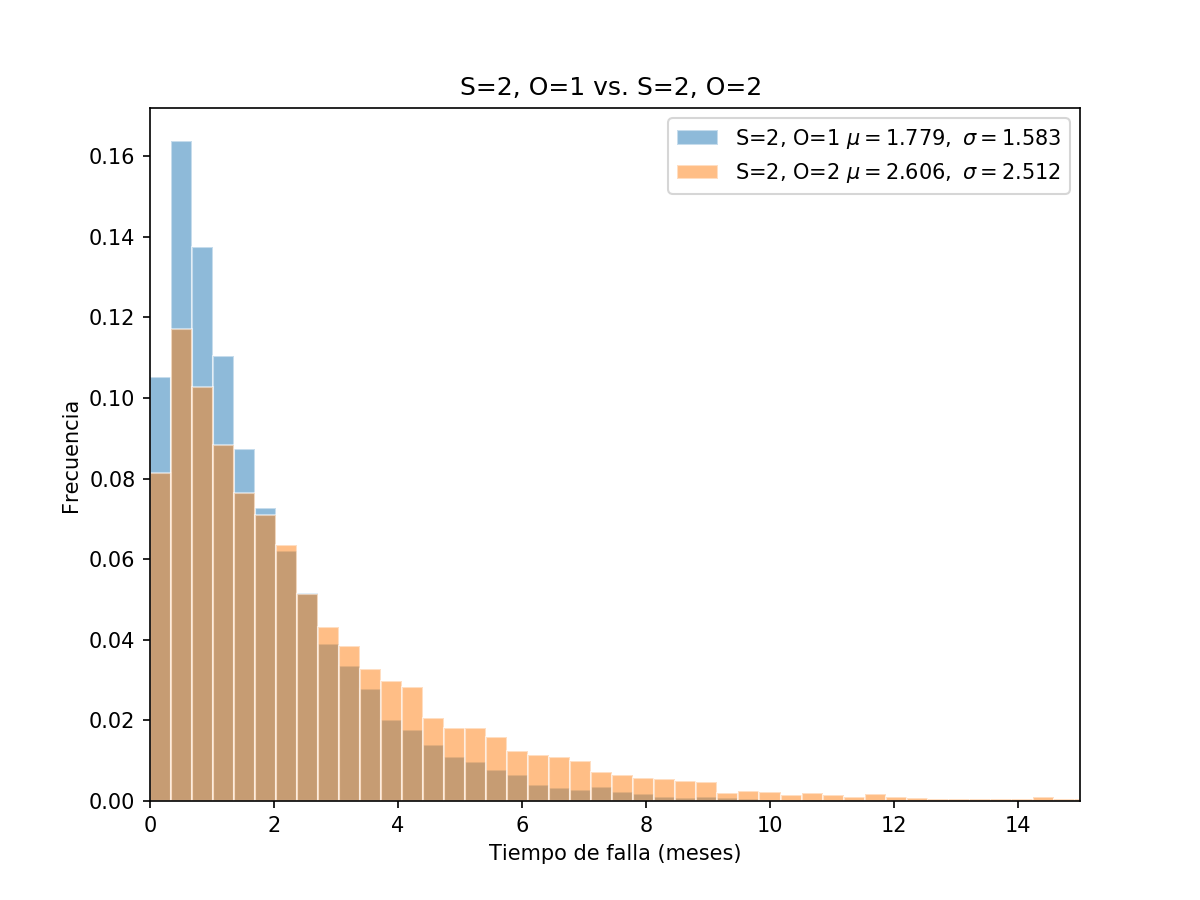
\includegraphics[scale=0.8]{images/S2O1vsS2O2.png}
        \caption{Histograma de comparación entre S = 2, O = 1 y S = 2, O = 2}
        \label{fig:S2O1vsS2O2}
    \end{figure}
    \vspace{5mm}

    \par En la Figura \ref{fig:S2O1vsS2O2} se puede observar que cuando se agrega un
    operario el tiempo esperado de falla
    del sistema aumenta considerablemente. Este resultado es el que esperábamos, pues
    aumenta la velocidad de reparación de máquinas al aumentar la cantidad de individuos
    capaces de reparar al mismo tiempo.

    \pagebreak

    \subsection{Comparación: Agregar una máquina}

    \par En este caso, realizamos una comparación de las tres situaciones antes
    mencionadas.
    \par Se ejecutó el algoritmo antes descripto con los conjuntos de parámetros
    correspondientes a las situaciones a comparar. Esto es:

    \[
      N = 5; \; T_F = 1; \; T_R = 0.125; \; S = 2; \; O = 1
    \]
    \[y\]
    \[
      N = 5; \; T_F = 1; \; T_R = 0.125; \; S = 3; \; O = 1
    \]


    \begin{figure}[h]
        \centering
        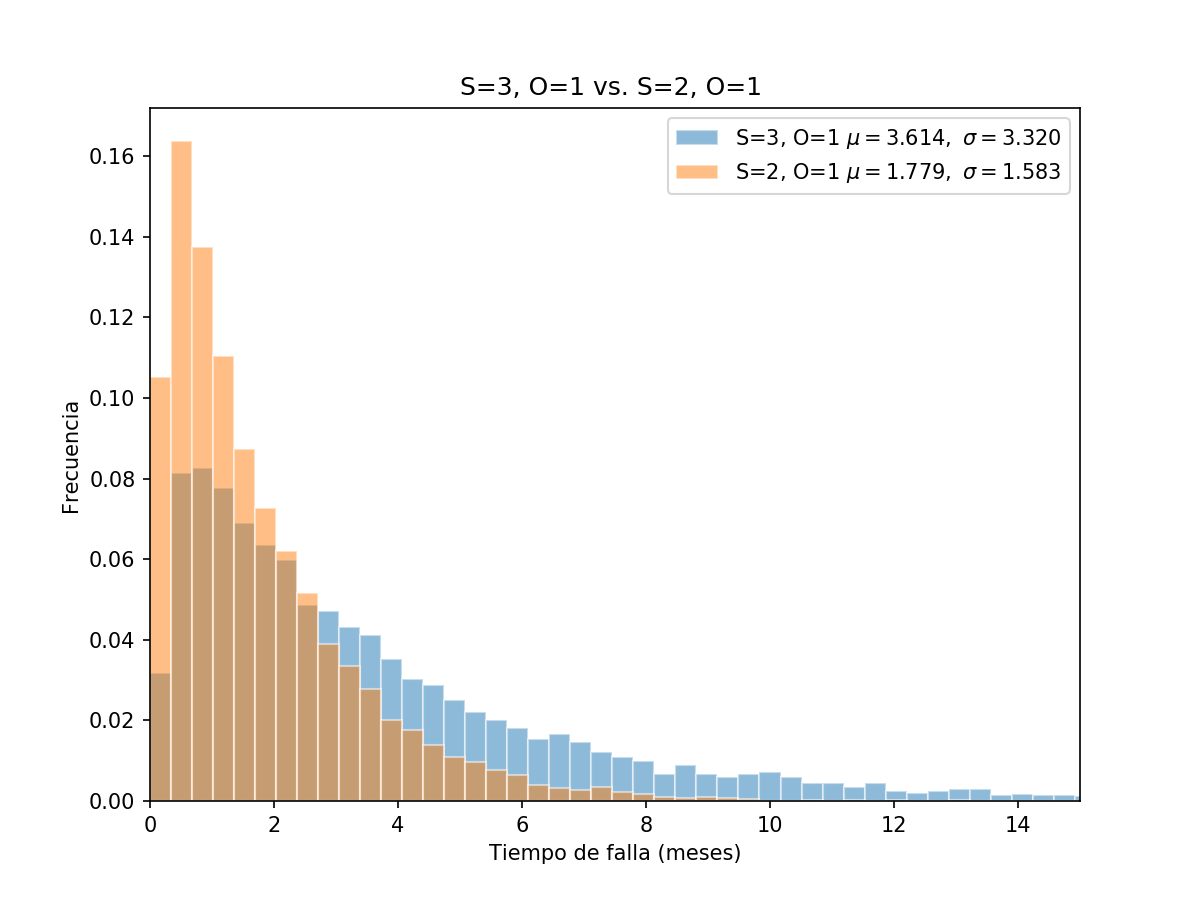
\includegraphics[scale=0.8]{images/S3O1vsS2O1.png}
        \caption{Histograma de comparación entre S = 2, O = 1 y S = 3, O = 1.}
        \label{fig:S2O1vsS3O1}
    \end{figure}
    \vspace{5mm}


    \par En la Figura \ref{fig:S2O1vsS3O1} se puede observar que cuando se agrega una
    máquina el tiempo esperado de falla
    del sistema aumenta considerablemente. Este resultado es el que esperábamos, pues al
    aumentar la cantidad de máquinas de repuesto los operarios tienen más tiempo para
    reparar las máquinas antes de que el sistema falle.

  \pagebreak

  \subsection{Comparación: Agregar una máquina vs. agregar un operario}

  \par En este caso, realizamos una comparación de la situación en que el lavadero
  tiene 3 máquinas de repuesto y 1 sólo operario con la situación en que tiene 2
  máquinas de repuesto y 2 operarios.
  Se ejecutó el algoritmo antes descripto con los dos conjuntos de parámetros
  correspondientes a las situaciones a comparar. Esto es:

  \[
    N = 5; \; T_F = 1; \; T_R = 0.125; \; S = 3; \; O = 1
  \]
  \[y\]
  \[
    N = 5; \; T_F = 1; \; T_R = 0.125; \; S = 2; \; O = 2
  \]

  \begin{figure}[h]
      \centering
      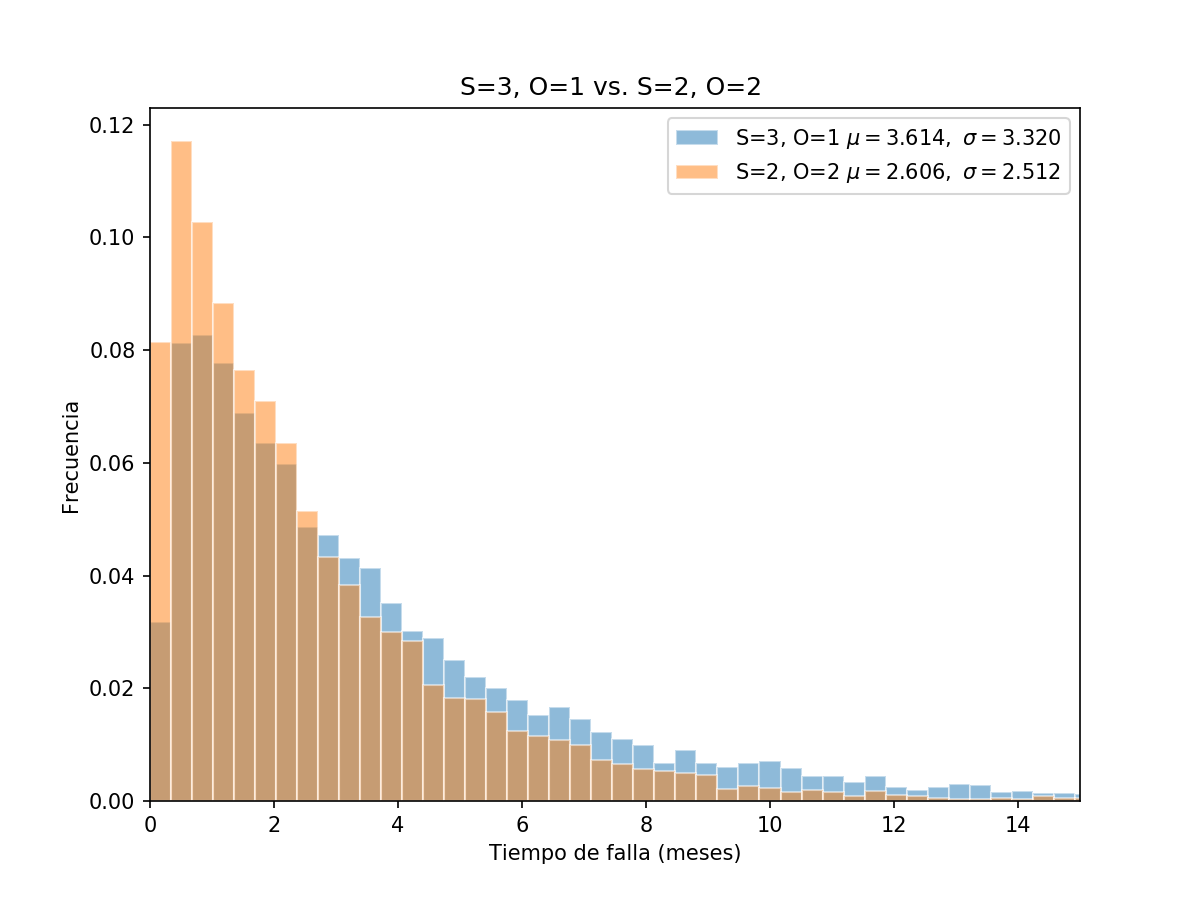
\includegraphics[scale=0.8]{images/S3O1vsS2O2.png}
      \caption{Histograma de comparación entre S = 3, O = 1 y S = 2, O = 2}
      \label{fig:S3O1vsS2O2}
  \end{figure}
  \vspace{5mm}

  \par En la Figura \ref{fig:S3O1vsS2O2} se puede observar que adquirir una máquina más
  de repuesto es más conveniente
  que contratar un operario extra pues el tiempo medio de falla del sistema aumenta.
  En particular, se puede notar en el histograma que la probabilidad de que el sistema falle
  dentro de los primeros 2 meses es considerablemente superior en el caso de que
  se contrata a un nuevo operario.
